\documentclass[a4paper,11pt]{report}
\usepackage{ragged2e}
\usepackage{float} 
\usepackage{subcaption}
\usepackage{fancyhdr}
\usepackage{graphicx}
\usepackage[top=1.5cm, bottom=3cm, left=2.5cm, right=2.5cm]{geometry} % Adjust margins
\usepackage{setspace}
\usepackage[linktoc=page]{hyperref}
\usepackage{sectsty}
\chapterfont{\centering}
\usepackage{makeidx}
\usepackage{url}
\usepackage[square,sort,comma,numbers]{natbib}
\usepackage{framed}
\usepackage{longtable}
\usepackage{amsfonts}
\usepackage{amsmath}
\usepackage{booktabs} % For better looking tables
\usepackage{array} 
\usepackage[noend,ruled,noline,linesnumbered,algochapter]{algorithm2e}

% Set header and footer space
\setlength{\headheight}{0pt} % Remove extra height in header
\setlength{\headsep}{0.5cm} % Reduce space between header and text

% Title Page
\begin{document}

% Fancy header and footer settings
\pagestyle{fancy}
\fancypagestyle{plain}{%
    \fancyhf{} % clear all header and footer fields
    \renewcommand{\headrulewidth}{0pt}
   
    \fancyfoot[R]{\thepage}
}

\fancyhf{} % clear all header and footer fields
\renewcommand{\headrulewidth}{0pt}

\fancyfoot[R]{\thepage}

% Set headers: chapter on the left, section on the right
\fancyhead[L]{\nouppercase{\leftmark}} % Chapter title on the left
\fancyhead[R]{\nouppercase{\rightmark}} % Section title on the right

% Title Page
\begin{titlepage}

\vspace*{2cm} % Adjust this value to increase the header space

\begin{center}
{\huge\bf Bicycle Management System}
\end{center}

\vspace{2cm}

\begin{center}
\Large \bf Submitted By
\end{center}

\vspace{.1cm}

\begin{table}[h!]
\centering
\begin{tabular}{|c|c|}
\hline
\textbf{      Student Name      } & \textbf{  Student ID  } \\
\hline
Jannatul Ferdaues & 232-15-689 \\
\hline
Tammam Ibn Aman & 232-15-755 \\
\hline
Nushrat Zahan Jui & 232-15-910 \\
\hline
\end{tabular}
\end{table}

\vspace{2cm}

\begin{center}
{\Large\bf BICYCLE MANAGEMENT SYSTEM LAB PROJECT REPORT}\\
\vspace{0.2cm}
\Large This Report Presented in Partial Fulfillment of the course  \textbf{CSE222: Object Oriented Programming Lab in the Computer Science and Engineering Department}
\end{center}

\vspace{2cm}

\begin{center}

\includegraphics[scale=0.5]{./figures/DIU Logo}
\end{center}

\begin{center}
	\Large\textbf{DAFFODIL INTERNATIONAL UNIVERSITY}\\
 \textbf{\textsc{Dhaka, Bangladesh}}
\end{center}

\begin{center}
\textbf{\today}
\end{center}

\end{titlepage}

\clearpage

% Set Roman page numbering for initial pages
\pagenumbering{roman}
\setcounter{page}{1}

% Declaration-------------------------
\phantomsection

\vspace*{1.5cm} 

\addcontentsline{toc}{chapter}{Declaration}

\begin{center}
    {\LARGE \textbf{DECLARATION}}\\
   % \line(1,0){430}
\end{center}

\onehalfspacing

\noindent We hereby declare that this lab project has been done by us under the supervision of \textbf{Md. Sazzadur Ahamed}, \textbf{Assistant Professor}, Department of Computer Science and Engineering, Daffodil International University. We also declare that neither this project nor any part of this project has been submitted elsewhere as lab projects. 

\vspace{.8cm}

\noindent \textbf{Submitted To:} \\[1cm]

\noindent\rule{6cm}{0.4pt}\\
\textbf{Md. Sazzadur Ahamed} \\
Designation Assistant Professor\\
Department of Computer Science and Engineering \\
Daffodil International University \\

\vspace{.5cm}

% Table
\begin{center}
    \textbf{Submitted by}
\end{center}

\vspace{.2cm}

\begin{table}[h!]
\centering
\renewcommand{\arraystretch}{3} % Increase row height for more space
\setlength{\tabcolsep}{10pt} % Adjust column spacing

\begin{tabular}{|p{0.48\textwidth}|p{0.35\textwidth}|} % Equal column widths

\hline
\multicolumn{2}{|c|}{
    \begin{minipage}{\linewidth}
        \centering
        \vspace{1.5cm} % Space above the name for signature
        \rule{6cm}{0.4pt} % Signature line
        \\
        \textbf{Jannatul Ferdaues} \\ 232-15-689 \\ Dept. of CSE, DIU
    \end{minipage}
} \\
\hline

\begin{minipage}{\linewidth}
    \centering
    \vspace{1.5cm} % Space above the name for signature
    \rule{6cm}{0.4pt} % Signature line
    \\
    \textbf{Tammam Ibn Aman} \\ 232-15-755 \\ Dept. of CSE, DIU
\end{minipage} &

\begin{minipage}{\linewidth}
    \centering
    \vspace{1.5cm} % Space above the name for signature
    \rule{6cm}{0.4pt} % Signature line
    \\
    \textbf{Nushrat Zahan Jui} \\ 232-15-910 \\ Dept. of CSE, DIU
\end{minipage} \\
\hline
\end{tabular}
\end{table}


\newpage
%Abstract
\phantomsection
\vspace*{1.5cm} 
\addcontentsline{toc}{chapter}{Course \& Program Outcome}
\setlength{\headheight}{14pt}
\begin{center}
	{\LARGE \bf COURSE \& PROGRAM OUTCOME}\\
	%\line(1,0){430}
\vspace*{1.5cm} 
\begin{flushleft}
The following course have course outcomes as following:.
\end{flushleft}

% table of CO's....................
\begin{table}[h!]
\centering
\caption{Course Outcome Statements}
\vspace{0.1cm} % Adds a 0.5 cm space between the caption and the table
\begin{tabular}{|p{0.06\textwidth}|p{.9\textwidth}|}
\hline
\textbf{CO's} & \textbf{Statements} \\
\hline
CO1 & \textbf{Define} and \textbf{Relate} To learn how to use programming languages (e.g., Java) and development tools (e.g., IDEs, Git) to build object-oriented systems, applying concepts like classes, inheritance  and polymorphism.
 \\
\hline
CO2 & \textbf{Formulate}To design and implement different system modules such as user management, bicycle booking and availability tracking, utilizing modern software development tools that are critical for building robust applications.
 \\
\hline
CO3 & \textbf{Analyze} To design and to analyze the performance and functionality of the system, focusing on data consistency, real-time updates and database interactions, ensuring efficient operations under various conditions and loads. \\
\hline
CO4 & \textbf{Develop} Involves and evaluate features such as user interfaces, backend logic and database management for the Bicycle Management System, using debugging tools and testing environments to ensure the system’s reliability and performance. \\
\hline
\end{tabular}
\end{table}

\vspace{1cm}
%----------------------------
% table for Mapping of CO, PO, Blooms, KP and CEP---------
\begin{table}[h!]
\centering
\caption{Mapping of CO, PO, Blooms, KP and CEP}
\begin{tabular}{|>{\centering\arraybackslash}m{2cm}|>{\centering\arraybackslash}m{2cm}|>{\centering\arraybackslash}m{2cm}|>{\centering\arraybackslash}m{2cm}|>{\centering\arraybackslash}m{2cm}|}
\hline
\textbf{CO} & \textbf{PO} & \textbf{Blooms} & \textbf{KP} & \textbf{CEP} \\
\hline
CO1 & PO1 & C1,P1,P2,P3 & KP1 & EP1,EP3 \\
\hline
CO2 & PO1,PO2 & C2,C3,P1,P2 & KP1,KP2 & EP2,EP3 \\
\hline
CO3 & PO3 & C3,P1,P2,P4 & KP3 &EP3 \\
\hline
CO4 & PO3 & C3, C6, P2 & KP3,KP4 & EP1,EP3 \\
\hline
\end{tabular}
\end{table}
\begin{flushleft}
The mapping justification of this table is provided in section \textbf{4.3.1}, \textbf{4.3.2} and \textbf{4.3.3}.
\end{flushleft}


\setlength
{\headheight}{12pt}


% Table of contents
\renewcommand*\contentsname{Table of Contents}
\tableofcontents
\clearpage

\renewcommand\bibname{References}
\clearpage

% Start of report and chapters
\pagenumbering{arabic} % Switch to Arabic numbering
\setcounter{page}{1}

% Reapply header and footer settings for the main content
\fancyhf{} % clear header and footer

\fancyfoot[R]{\thepage}
\fancyhead[L]{\nouppercase{\leftmark}} % Chapter title on the left
\fancyhead[R]{\nouppercase{\rightmark}} % Section title on the right

% Chapters content...................................
\chapter{Introduction}
A Bicycle Management System is a digital platform that helps manage bicycle rentals and inventory. It stores user and bicycle data, tracks availability, and handles check-ins and check-outs. This system streamlines operations, allowing users to easily rent bicycles while providing admins with efficient control over the fleet.
\justifying
\section{Introduction}
The Bicycle Management System offers a smart and organized way to oversee bicycle rentals and inventory through a digital solution. Acting as a strong example of automation in resource management, this system simplifies the tasks of checking bicycle availability, handling rentals and maintaining usage logs within a single platform. It demonstrates how digital tools can effectively replace outdated manual systems, making operations more efficient and user-friendly.
This system keeps track of user data, bicycle status and rental records, allowing users to easily rent or return bicycles while giving administrators full control over monitoring and managing the fleet. Built using simple database technology and an intuitive interface, it is both cost-efficient and easy to implement across different environments.
The Bicycle Management System is particularly useful for bike-sharing programs, educational institutions and urban transport networks where structured bicycle usage is essential. Moreover, it encourages sustainable transportation habits and offers a convenient solution for users, providing quick access and smooth service with minimal effort.\cite{1.1}

\subsection{Problem Statement} Managing bicycle rentals through conventional means like manual entries, paper-based logs, or verbal coordination can be functional but often lacks efficiency, accuracy and ease of use. Such traditional systems are not well-suited to modern needs, especially in environments with high user volume or frequent bicycle turnover. Users may struggle to find available bicycles, while administrators face difficulties tracking usage, ensuring proper maintenance and avoiding scheduling conflicts. These limitations highlight the need for an automated system to improve workflow and user experience. However, implementing such a solution comes with several key challenges:
\begin{itemize}
    \item \textbf{Real-Time Data Management} The system must maintain up-to-date information on bicycle status, ensuring users and administrators have access to accurate availability records.
    \item \textbf{Ease of Use and Accessibility:} It’s important that the platform is user-friendly and accessible to a wide range of users, including those with minimal technical experience.
    \item \textbf{System Expansion and Load Handling:} The solution should be capable of supporting future growth, handling more bicycles and users without performance issues.
    \item \textbf{Infrastructure Compatibility:} To be widely adopted, the system should be flexible enough to integrate smoothly with existing environments, whether in educational institutions, corporate spaces, or public transport networks.\cite{1.1.1}\\

\end{itemize}

\section{Motivation}
With growing emphasis on sustainable and cost-effective transportation, bicycles have emerged as a preferred mode of travel in many urban and institutional settings. Despite this, the lack of an efficient and structured system for managing bicycle rentals often leads to confusion, unavailability and maintenance delays. Manual processes are time-consuming and inefficient, especially when dealing with large volumes of users and bicycles.\\

\noindent The core motivation for creating a Bicycle Management System stems from the need to automate and simplify these operations. By providing a centralized digital platform, the system can facilitate real-time bicycle tracking, streamlined rentals, and improved maintenance scheduling. This enhances the overall user experience while offering administrators greater visibility and control.Ultimately, this project aims to replace outdated manual methods with a reliable, scalable, and smart solution tailored for modern transportation needs.\cite{1.2}

\section{Objectives}
The primary aim of this project is to design and implement a digital system that simplifies the process of renting and managing bicycles. This system seeks to replace traditional manual methods with an automated, user-friendly platform that improves efficiency, accuracy and user satisfaction.
\item \textbf{The objectives of this project are to:}
\begin{itemize}
\item To create a web-based interface that allows users to view available bicycles and make rental requests.
\item To develop an admin panel for managing bicycle inventory, tracking rentals and scheduling maintenance.
\item To ensure secure storage of user and transaction data using a reliable database system.
\item To enhance the overall experience for both users and administrators by minimizing manual workload and reducing errors.
\item To support scalability, allowing the system to accommodate more users and bicycles in the future.\cite{1.3}
\end{itemize}

\section{Feasibility Study}
The Bicycle Management System project is centered around creating a structured, low-cost, and efficient digital solution for managing bicycle rentals and inventory through a web-based platform. It leverages fundamental technologies such as relational databases, server-side programming and front-end interfaces to streamline rental processes and inventory tracking. \\
\item \textbf{Similar Research and Case Studies:}
Numerous studies and implemented systems have demonstrated the effectiveness of digital platforms in managing shared resources, such as library systems, vehicle rental services and campus equipment tracking. These projects commonly incorporate user registration, asset availability tracking and transaction history logging features also fundamental to the Bicycle Management System. The success of such systems in academic and commercial environments validates the feasibility of applying similar methodologies to bicycle sharing and rental services.
\item \textbf{Methodological Contributions from Existing Projects:}
Prior projects in asset management and rental systems have laid the groundwork for the development of scalable, modular software solutions. Key methodologies adopted include session-based user management, MySQL-based data handling and admin dashboards for backend control. While more advanced platforms might incorporate AI or IoT-based tracking, the foundational approach of using structured databases and clean UI design has remained effective in many successful implementations.
\item \textbf{Web Applications:}
Though primarily designed for desktop platforms, the system’s architecture is flexible enough to allow for integration with future mobile or web applications if needed. Desktop-based solutions for resource management are especially beneficial for organizations that do not require high mobility or constant internet access. Furthermore, desktop applications offer offline capabilities, which could be advantageous in environments with unreliable internet connections.\cite{1.4}

\section{Gap Analysis}
The Bicycle Management System addresses the limitations of traditional bicycle rental methods, which are often inefficient and manually intensive. While digital rental platforms exist, they are typically costly or not tailored for bicycle-sharing programs. This project fills the gap by offering an affordable, user-friendly solution that streamlines the rental process and integrates secure online payment options. It aims to provide a practical, scalable system for both large and small bike-sharing programs, promoting easier access to sustainable transportation.\cite{1.5}


\section{Project Outcome}
The Bicycle Management System delivers a fully functional platform that streamlines the process of managing bicycle rentals and inventory. It simplifies user interactions by allowing easy bicycle reservations and management through an intuitive web interface, eliminating the need for manual tracking and physical paperwork. This system increases convenience, accessibility and efficiency, making bicycle-sharing programs more user-friendly and organized.\\
Additionally, the project demonstrates the practical use of web development, database management and payment gateway integration in real-world applications, showcasing how simple technologies can work together to create effective solutions. Moreover, the development of the Bicycle Management System enhances skills in software development, database handling and user interface design, bridging theoretical knowledge with real-world execution. It encourages problem-solving, creative thinking, and the application of technology to address real-life challenges, inspiring further innovations in digital systems for transportation management.\cite{1.6}

\subsection{Program Outcome List}
\begin{itemize}
    \item \textbf{Engineering Knowledge:} Utilizes software development principles and database management to create a robust system for bicycle rental and inventory management.
\item \textbf{Problem Analysis:} The project involves detailed analysis of the challenges in managing bike-sharing services and designing practical solutions for users and administrators.
\item \textbf{Design Solutions:} Develops a fully functional digital platform that automates the rental process, streamlining the user experience and improving system efficiency.
\item \textbf{Teamwork:} The project encourages collaboration among team members, with everyone contributing to the design, development, and testing phases.
\item \textbf{Communication:} Enhances skills in presenting project ideas clearly and documenting the development process for effective communication with stakeholders.
\item \textbf{Project Management:} Develops planning and resource allocation skills: Strengthens abilities in planning, scheduling, and resource management to ensure the timely completion of the project.
\end{itemize}


\chapter{Proposed Methodology}
The Bicycle Management System is a smart project that automates bicycle rentals using a web platform. It applies object-oriented programming to manage users, track bicycles and handle reservations, making it ideal for learning real-world software development.

%This is for reference only. Delete before finalization


\section{Requirement Analysis \& Design Specification} The Bicycle Management System aims to simplify and digitize the process of renting, returning and tracking bicycles. During the requirement analysis, both functional and non-functional needs of the system were identified. Functional requirements include user registration, login authentication, viewing available bicycles, booking and returning cycles. Admin-specific features include managing bicycle inventory, tracking usage and viewing system reports.\\
The design specification phase focused on building a structured system using object-oriented principles, with clear definitions of classes such as User, Admin, Bicycle, and Booking. The system was designed with a responsive user interface and a MySQL database for reliable data storage and retrieval. Security, scalability and ease of use were also key considerations to ensure the system performs well in real-world environments like campuses or public bike-sharing programs.
\cite{2.1.1}

\subsection{Overview}
The diagram for the Bicycle Management System illustrates a basic web-based platform that allows users to manage bicycle rentals efficiently. Users interact with the system through a login portal, where they can view available bicycles, book a ride and return bicycles after use.\\
The system processes these actions using a backend database, typically MySQL, which handles data related to users, bicycles and bookings. Object-oriented components such as User, Bicycle, and Reservation classes interact to maintain smooth operations.\\
This project offers an easy and user-friendly way to handle bike-sharing tasks, promoting organized, hands-free management through a digital interface.\cite{2.1.3}

\subsection{Proposed Methodology}
\begin{itemize}
\item \textbf{User Interaction:} Users access the system through a web interface where they can register, log in and manage their bicycle rentals.
\item \textbf{Data Processing:} Once a user makes a request (such as booking a bicycle), the system processes it using backend logic implemented with object-oriented programming concepts.
\item \textbf{Database Management:} The system uses a MySQL database to store and retrieve data related to bicycles, users and bookings. All interactions are logged and updated in real-time for accuracy.
\item\textbf{Booking Confirmation:} When a booking is confirmed, the system updates the bicycle’s status and ensures it is marked as unavailable until returned.
\item \textbf{System Hosting: } The application runs on a local server or web host, supported by a stable backend framework and database connection, ensuring smooth and efficient operation of all modules.\cite{2.1.1}
\end{itemize}

\begin{figure}[h] % 'h' for placing it "here"
\subsection{UML Design}
    \centering
    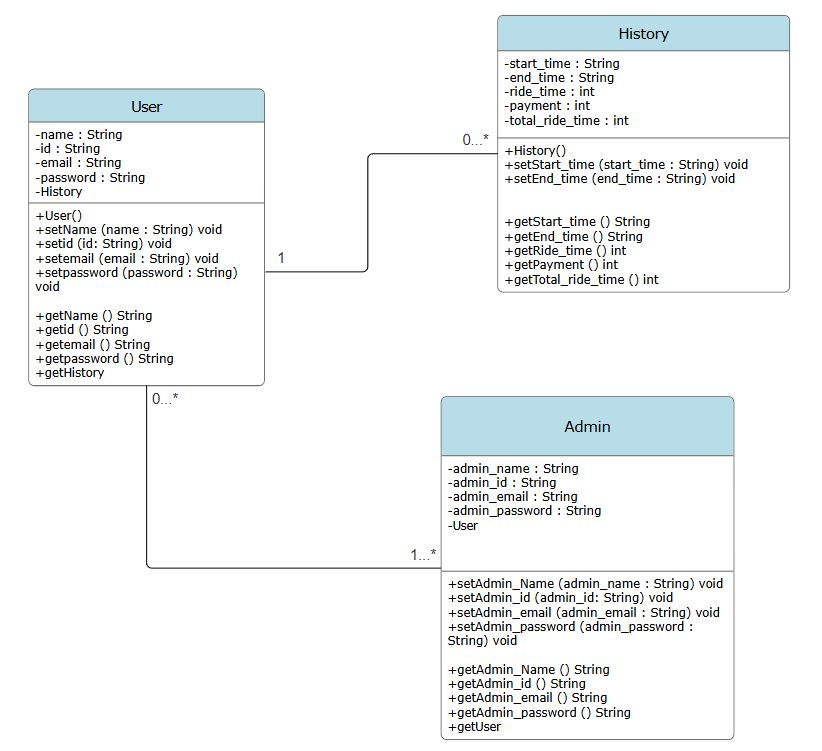
\includegraphics[width=0.9\textwidth]{figures/Others/UML.jpg} % Replace 'UML.jpg' with your image file
    \caption{UML}
    \label{fig:sample}
\end{figure}


\subsection{Frontend Design}
\begin{figure}[H]
    \centering
    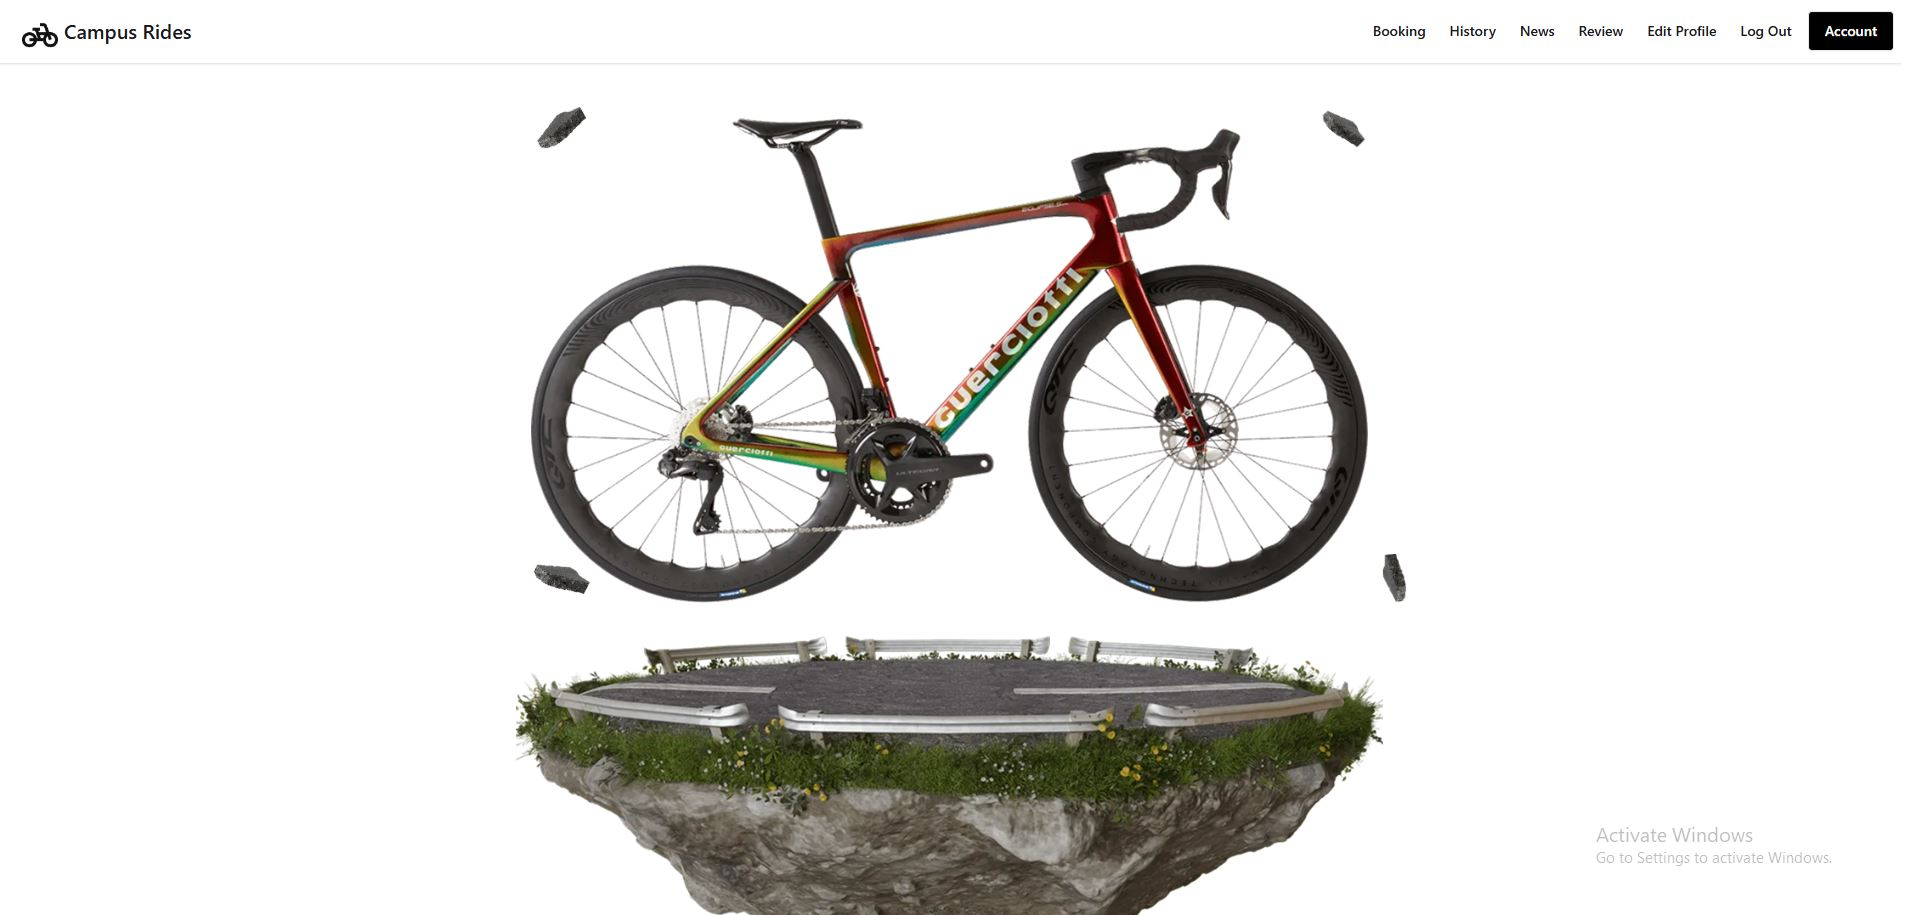
\includegraphics[width=0.6\textwidth]{figures/UI/home.jpg} % Replace with your image path
    \caption{Home Page}
    \label{fig:sample}
\end{figure}
\begin{figure}[H]
    \centering
    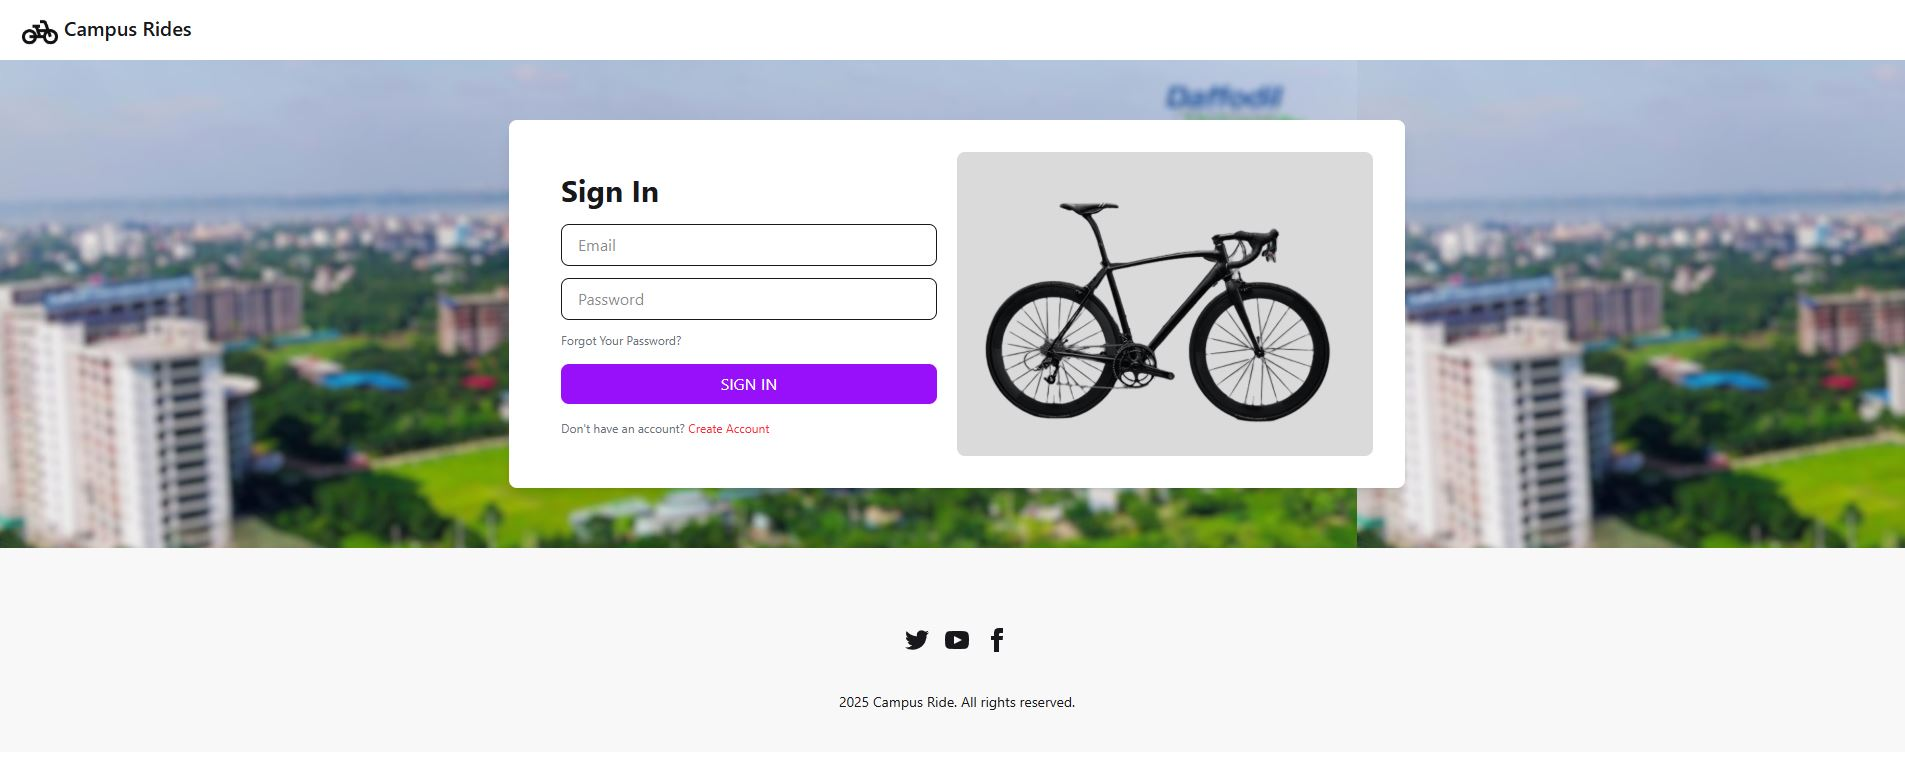
\includegraphics[width=0.6\textwidth]{figures/UI/log_in.jpg} % Replace with your image path
    \caption{Login Page}
    \label{fig:sample}
\end{figure}
\begin{figure}[H]
    \centering
    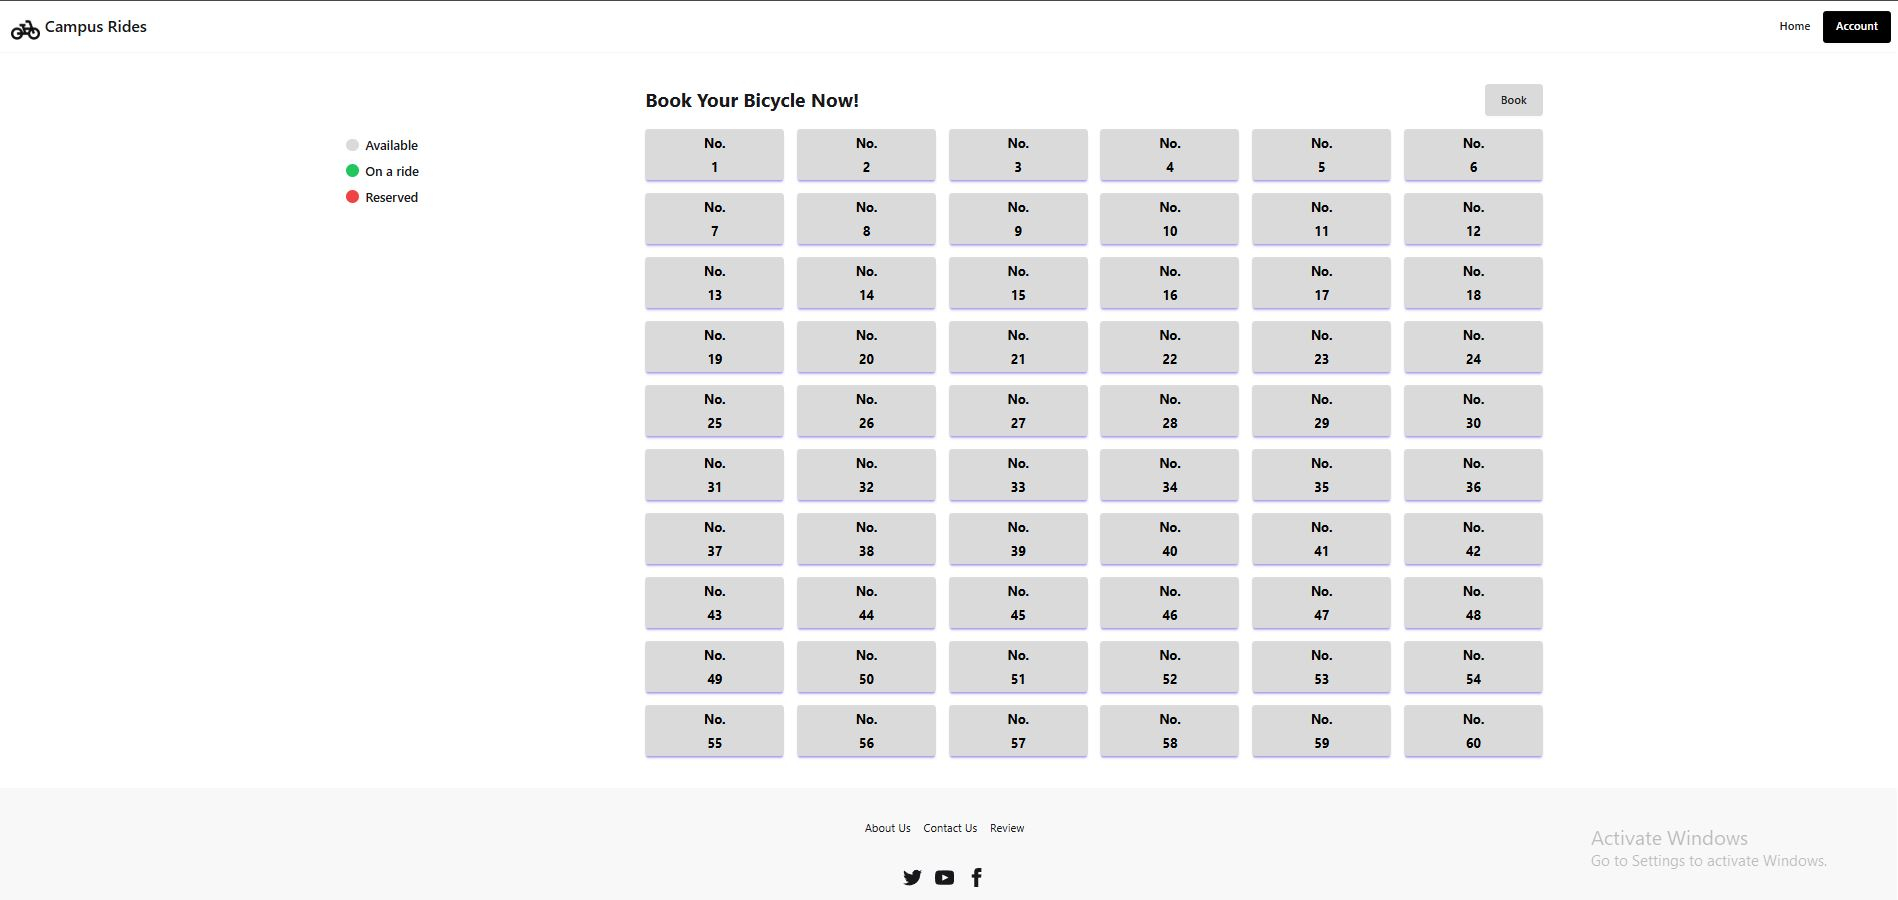
\includegraphics[width=0.5\textwidth]{figures/UI/booking.jpg} % Replace with your image path
    \caption{Booking Page}
    \label{fig:sample}
\end{figure}
\begin{figure}[H]
    \centering
    \includegraphics[width=0.9\textwidth]{figures/UI/timer.jpg} % Replace with your image path
    \caption{Timer Page}
    \label{fig:sample}
\end{figure}
\begin{figure}[H]
    \centering
    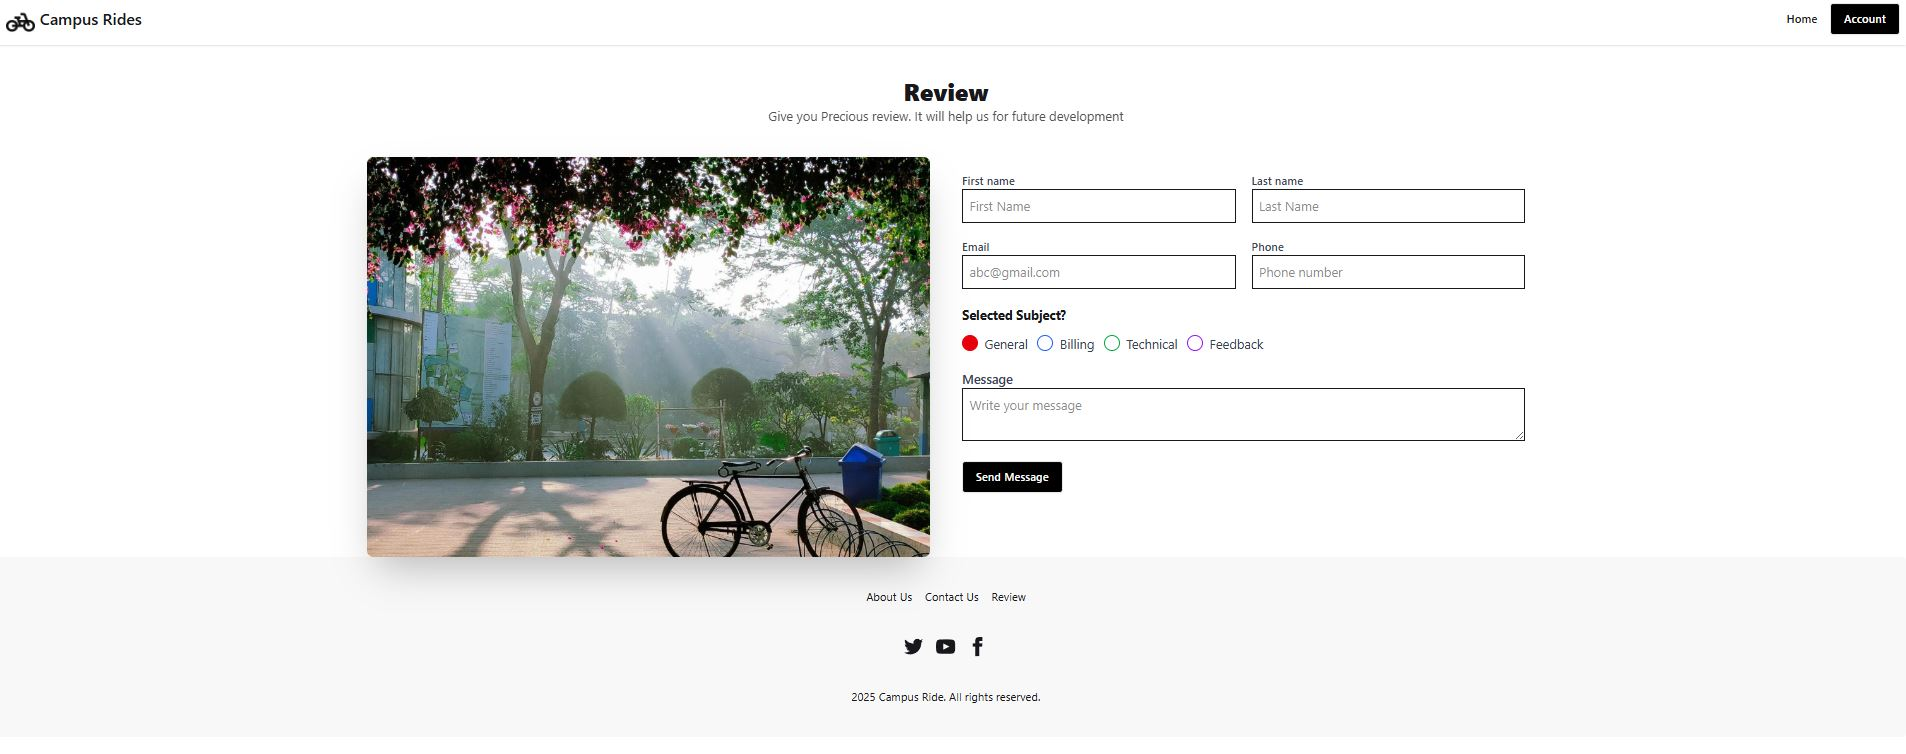
\includegraphics[width=0.7\textwidth]{figures/UI/review.jpg} % Replace with your image path
    \caption{Review Page}
    \label{fig:sample}
\end{figure}
    
\section{Overall Project Plan}
The Bicycle Management System Project focuses on creating a web-based platform to efficiently manage shared bicycles. The project will move through phases including research, design, hardware selection, web development, testing and improvement based on user feedback.\\

\noindent The system will use components like GPS modules, RFID/NFC tags and microcontrollers to monitor bicycle location and usage. A web application will be developed to handle user registration, bicycle tracking and real-time status updates.\\

\noindent All management functions such as checking availability, assigning bicycles  and viewing usage history will be accessible through the web interface. Testing will ensure the system is accurate, secure and user-friendly. The goal is to deliver a practical and reliable bicycle management solution without relying on mobile apps.\cite{2.2}\\

\begin{table}[h!]
\subsection{Time Frame}
\centering
\begin{tabular}{|l|c|c|c|c|}
\hline
\textbf{Working Days}              & \textbf{Analysis+Content Ready} & \textbf{Frontend} & \textbf{DataBase} & \textbf{Backend} \\ \hline
Week 1 & \checkmark              &                 &                 &                 \\ \hline
Week 2             & \checkmark            &  \checkmark               &                 &                 \\ \hline
Week 3        &               &  \checkmark               &                 &   \checkmark               \\ \hline
Week 4        &                &              & \checkmark                 &    \checkmark              \\ \hline
Week 5        &                &              &   \checkmark               &   \checkmark               \\ \hline
Week 6      &                &                 & \checkmark              &   \checkmark               \\ \hline
\end{tabular}
\caption{Project Schedule.}
\label{tab:project_schedule}
\end{table}


\chapter{Implementation and Results}
This chapter explores the development and outcomes of the Bicycle Management System, focusing on its effective tracking functionality, simple and accessible interface and suitability for various use cases, while also considering existing challenges and future improvements for better dependability.
\end{center}

%This is for reference only. Delete before finalization

\section{Implementation}
The Bicycle Management System is designed to monitor and manage bicycle usage efficiently through a digital interface. Core components include a user registration module, database connectivity (using MySQL) and a responsive frontend. Backend functionalities are implemented using Spring Boot, while MySQL handles data storage and retrieval.
Users can register, log in and track bicycle usage or availability. Admins can manage bicycle records, user details  and usage history. The system ensures smooth data flow between frontend and backend, supporting real-time updates and interactions, making it suitable for campus or community bicycle programs.\cite{3.1}

\section{Performance Analysis}
The Bicycle Management System delivers effective and organized control over bicycle access and tracking. It ensures smooth performance through optimized database queries and secure login systems.\\
The system is scalable and flexible, with the ability to integrate additional features like QR scanning or GPS tracking. Challenges may arise from connectivity issues or database load under high usage, but these can be mitigated through optimization and error handling.
The project combines reliability with user convenience, making it a practical solution for sustainable transport management in smart campuses or eco-friendly communities.\cite{3.2}

\section{Results and Discussion}
The Bicycle Management System effectively manages and monitors bicycle usage through a digital platform. Testing confirmed smooth operation of core features such as user registration, login authentication and real-time bicycle tracking. The system performed reliably under normal usage conditions, with minor delays observed only under high network load or database congestion, indicating areas for optimization.\\
The integration of MySQL with Spring Boot ensured stable data handling, while the frontend provided a responsive and user-friendly experience. Admin functionalities, such as bicycle allocation and usage history monitoring, worked as intended without critical issues.\\
Overall, the system proved to be reliable, efficient, and adaptable. With potential upgrades like GPS integration or mobile app support, the project can be further enhanced for broader usage in campuses, communities, or rental services, supporting eco-friendly transportation solutions.\cite{3.3}\\


\chapter{Engineering Standards and Mapping}
%This is for reference only. Delete before finalization
The Bicycle Management System follows engineering standards by ensuring secure data management, reliable performance and user-friendly access, with proper design, testing and user input to meet key functional and security needs.

\section{Social and Environmental Sustainability}
The Bicycle Management System contributes to social and environmental sustainability by promoting eco-friendly transportation and encouraging healthier, more active lifestyles. By making bicycle access and tracking more organized and efficient, it supports communities in reducing their carbon footprint and traffic congestion.
This system enhances mobility for students, employees and community members, offering a cost-effective and sustainable alternative to motorized transport. It is especially beneficial in campuses or urban areas where short-distance travel is common. Additionally, the digital nature of the system supports inclusive access and convenience, allowing users to locate and use bicycles with minimal effort.
However, its impact depends on accessibility, technological literacy and infrastructure. Limited digital access or lack of user awareness could affect its effectiveness. Overreliance on automated systems might also reduce personal responsibility in managing shared resources.\\
Overall, the Bicycle Management System aligns with modern sustainability goals, encouraging green habits and efficient transport solutions, while requiring thoughtful implementation to ensure broad accessibility and long-term societal benefit.
\cite{4.1}


\subsection{Impact on Life}
\textbf {Convenient Mobility:} The Bicycle Management System simplifies transportation by allowing users to easily locate, access and manage bicycles without the need for manual tracking. This promotes a more organized and accessible commuting experience, especially in campuses, offices and public areas.\\
\textbf{Time Efficiency:}With real-time data and digital access, users can quickly find available bicycles and avoid delays. This system is especially helpful in busy environments where time-saving is essential.\\
\textbf{Safety and Accessibility:}Organized bicycle access reduces clutter and potential hazards in shared spaces. In emergency or crowded situations, users can rely on the system to find safe and immediate transport options.\\
\textbf{Challenges:}Limited infrastructure, such as lack of dedicated bike lanes or storage areas, can reduce effectiveness. Some users may face difficulties adapting to the digital platform, especially those less familiar with technology. In addition, overdependence on automated systems may reduce users’ initiative in managing shared resources manually. The system may also need further enhancement to manage large-scale usage or multi-location operations.\cite{4.1.1}

\subsection{Impact on Society \& Environment}
The Bicycle Management System has a significant impact on both society and the environment. It encourages the use of bicycles as a primary mode of transport, promoting healthier lifestyles and reducing dependency on fuel-powered vehicles. This contributes to improved public health and decreased air pollution in urban and institutional environments.\\
Socially, it enhances mobility for individuals across different backgrounds, especially those who may not afford private transportation. By offering organized access and real-time tracking, it supports inclusivity and convenience, especially in educational institutions or urban communities.\\
Environmentally, the system supports sustainable transportation goals by reducing carbon emissions and traffic congestion. However, digital infrastructure and electronic device usage carry environmental considerations, such as energy consumption and e-waste from outdated systems. Proper management of digital waste and the use of energy-efficient servers and systems are essential for minimizing long-term environmental impact.\cite{4.1.2}
\subsection{Ethical Aspects}
The Bicycle Management System raises several ethical considerations including accessibility, data privacy, environmental impact and social equity. By offering an organized and efficient transportation method, the system supports inclusion and independence for a wide user base.
However, concerns about user data privacy must be addressed, particularly in systems that store personal information or track usage behavior. Secure handling, transparency in data processing and consent-based access are key ethical responsibilities.
From an environmental standpoint, the development and maintenance of the system should aim to minimize waste and power usage. Using sustainable software practices and durable hardware can reduce environmental harm.
Furthermore, the pricing and availability of such systems must consider social fairness. High costs or restricted access could disadvantage certain communities. Ethical deployment ensures that the technology remains accessible and beneficial across different socioeconomic groups without fostering inequality or overdependence on digital systems.\cite{4.1.3}
\subsection{Sustainability Plan}A sustainability plan for the Bicycle Management System incorporates environmental, social and economic goals throughout its development and deployment lifecycle. From the design phase, efforts should be made to use cloud services with low carbon footprints and efficient database systems to reduce energy use.
The backend infrastructure should be optimized for minimal energy consumption, while the frontend should be lightweight and accessible on low-end devices. Economically, offering multiple access levels free or subsidized options for students or low-income users helps ensure broader adoption.\\
Socially, promoting awareness campaigns and user education can drive responsible and effective use of the system. Long-term maintenance and updates should be planned with modular designs and scalable architecture to extend the system’s lifespan and reduce unnecessary upgrades or replacements.
At the end-of-life stage, decommissioning the system should include responsible disposal of physical devices and secure deletion of user data. Together, these steps ensure that the Bicycle Management System aligns with long-term sustainability and user satisfaction.\cite{4.1.4}

%\section

\section{Project Management and Team Work}
The Bicycle Management System was developed through effective team collaboration, with clear role distribution across design, frontend, backend and database management. A cost-effective version can be built using open-source technologies and local servers, suitable for educational or small-scale community projects. Revenue generation may come from three streams: subscription models for institutions, advertising or partnerships with local bike vendors. Projected revenue from 1,000+ active users or installations across universities and offices ensures a balanced approach to affordability and scalability, maintaining both social impact and financial sustainability.\cite{4.2}

\section{Complex Engineering Problem}
\textbf{Problem Statement:} Managing bicycle rentals or access in a large-scale system can be complex, especially when tracking multiple users, bicycles and usage history. Traditional manual systems may lead to inefficiencies, confusion and challenges in maintaining real-time data, particularly when managing access, availability and tracking in environments like universities or urban communities.\\
\textbf{The suggested Solution:}
The Bicycle Management System offers a solution by digitally organizing and automating bicycle access through a web-based platform. Users can register, log in and check the availability of bicycles in real time. The system is built using Object-Oriented Programming (OOP) principles, ensuring modularity, scalability and reusability in the codebase.\\
\textbf{Key Features of the Solution:}
\begin{itemize}
\item User Authentication and Role Management using OOP classes to ensure secure access and individualized privileges.
\item Bicycle Tracking with real-time updates, allowing users to view available bicycles based on location and status.
\item Efficient Database Management using OOP methods to interact with MySQL, ensuring smooth data retrieval and updates without redundancies.
\item Admin Control for managing user accounts, bicycle maintenance, and usage history.\cite{4.3}
\end{itemize}

\subsection{Mapping of Program Outcome} 
\textbf{Problem Statement:}
The manual operation of bicycle rental systems, particularly in large institutions or public spaces, can be time-consuming and inefficient. Users may face difficulties in locating available bicycles, while administrators may struggle with managing real-time data, user tracking and system updates. A traditional, non-automated approach can lead to delays and inaccurate information.\\
\textbf{The suggested Solution:}
The Bicycle Management System is a digital solution that automates the bicycle rental process, enabling users to easily locate, reserve, and rent bicycles through a web-based platform. Built with Object-Oriented Programming (OOP) principles, the system offers a modular, scalable design that allows for real-time updates, user authentication, and efficient resource management. By automating the system and using object-oriented principles, the platform simplifies management for both users and administrators.\\
\textbf{Key Features of the Solution:}
\begin{itemize}
\item Real-time data is updated and processed through efficient object interactions, allowing users to view available bicycles.
\item Admin users can monitor and manage bicycles, users, and usage logs, ensuring smooth operations.
\item MySQL is used with OOP methods to store, retrieve and manage data, ensuring smooth and error-free interactions.
\item The design supports both small-scale implementations for local setups and large-scale applications for city-wide bike-sharing systems.\cite{4.3.1}
\end{itemize}

\begin{center}
    \begin{table}[ht]
    
        \begin{tabular}{|p{0.2\textwidth}|p{0.7\textwidth}|}
            \hline
            \textbf{PO's} & \textbf{Justification} \\
            \hline
            PO1 & Demonstrates the application of fundamental software engineering principles, focusing on object-oriented design for creating a scalable, maintainable system. \\
            \hline
            PO2 & Effectively determines the requirements of users (both end-users and administrators) and implements a practical, intuitive solution that meets their needs.\\
            \hline
            PO3 & Designs and develops a functional bicycle management system, using object-oriented programming principles to ensure modularity and long-term maintainability. This system addresses real-world challenges like bicycle availability, tracking and user management.\\
            \hline
        \end{tabular}
        \centering
        \caption{Justification of Program Outcomes.}
        \label{tab:po_justification}
    \end{table}
\end{center}

\begin{center}
    \begin{table}[ht]
    \subsection{Complex Problem Solving} 
        \begin{tabular}{|p{0.12\textwidth}|p{0.12\textwidth}|p{0.12\textwidth}|p{0.12\textwidth}|p{0.12\textwidth}|p{0.12\textwidth}|p{0.12\textwidth}|}
        \hline
        EP1& EP2& EP3& EP4& EP5& EP6& EP7\\
        Dept of Knowledge & Range of Conflicting Requirements & Depth of Analysis & Familiarity of Issues & Extent of Applicable Codes & Extent of Stakeholder Involvement & Inter-dependence\\
        \hline 
         The project requires knowledge of the project involves expertise in OOP, software architecture and database management. Main challenges include ensuring data integrity, real-time updates and a smooth user interface, which are tackled using modular design and OOP techniques.
&The project requires involves balancing data accuracy and system efficiency, minimizing booking errors and availability conflicts. Key skills include programming, database management, algorithm design and object-oriented programming. Effective data processing is critical for optimal real-world performance.
 &The project involves moderate software integration, focusing on reliable system functionality. Key skills include OOP design, database management, API integration and interface development. Balancing cost and performance is essential, addressing challenges like data synchronization and system responsiveness common in software development.
&Testing involves common challenges like debugging software errors and adjusting system logic. The system must balance performance with user-friendliness, being both responsive and reliable in different conditions. Identifying bugs and refining features are crucial for optimal system performance.
&The project involves multiple segments of code that collectively implement the system’s functionality. The extent of applicable codes covers the full structure of the application using Object-Oriented Programming principles, ensuring modularity, reusability and scalability.
&The success of the Bicycle Management System relies heavily on the active involvement of stakeholders throughout the project lifecycle. Stakeholders contribute to defining requirements, guiding development and ensuring the system meets real-world needs.
&In this project involves a network of interrelated modules that must work in harmony. From booking bicycles to tracking returns and calculating costs, each part depends on the smooth functioning of the others, making inter-dependence a core aspect of the system’s design.
\\
        &&&&&&\\
        \hline 
        \end{tabular}
         \centering
        \caption{Mapping with complex problem-solving.}
        \label{tab:p_solve}
    \end{table}
     
\end{center}

\begin{center}
    \begin{table}[ht]
    \subsection{Engineering Activities}
    
        \begin{tabular}{|p{0.18\textwidth}|p{0.18\textwidth}|p{0.18\textwidth}|p{0.18\textwidth}|p{0.18\textwidth}|}
        \hline
        EA1& EA2& EA3& EA4& EA5\\
        Range of resources & Level of Interaction & Innovation & Consequences for society and environment & Familiarity\\
        \hline 
         Simpler resources, such as databases, programming languages (e.g., Java) and development tools, are used. The project requires cooperation between software developers and database administrators. Typical components include user interfaces and backend systems, with creativity focused on designing algorithms for booking management and bicycle availability.
         &Low engagement in component choice as it can be a solo task, though cooperation with database providers or software tools may be needed. Accessibility of development tools (e.g., IDEs, frameworks) is important. While the tools themselves require little creativity, the design of the system architecture and user experience is where the creative effort lies in combining these components into a functional system.

         &Creative algorithms and data handling methods are needed for managing bicycle availability and booking systems. Software tools (e.g., IDEs, database management tools) are used for modeling and implementation, along with physical components like user interfaces. High engagement between frontend design and backend logic is required, as the programming must align with system architecture for efficient functioning.
         &The project emphasizes efficiency and system reliability, which can have positive effects on user experience. Environmental issues are minimal if data privacy practices are followed. Testing tools (e.g., debuggers, unit tests) and a proper testing environment are crucial. Algorithm optimization for bicycle booking and availability management is important for enhancing performance and user satisfaction.
         &This project involves designing a Smart Bicycle Booking System using Object-Oriented Programming, where creative algorithms and effective data handling are essential for managing real-time bicycle availability, bookings and returns.
         \\
        &&&&\\
        \hline 
        \end{tabular}
        \centering
                \caption{Mapping with complex engineering activities.}
        \label{tab:e_act}
    \end{table}
\end{center}

\chapter{Conclusion}

%This is for reference only. Delete before finalization

This chapter presents an overview of the Bicycle Management System project, highlighting the key objectives, the methodology adopted and the results obtained. It addresses the challenges faced during development and proposes future improvements aimed at enhancing the system’s functionality, dependability, and scalability.

%This is for reference only. Delete before finalization

\section{Summary}
\textbf {Summary:} The aim of the Bicycle Management System project is to offer an efficient and user-friendly method for organizing and monitoring bicycle usage through a digital solution. The system incorporates essential elements such as user registration, bicycle availability tracking, booking options, and data management. Tools used include backend services, a database, and a responsive frontend interface. The application was designed to facilitate easy access and control over bicycle-related operations. Although the system successfully performed core tasks like managing bookings and displaying status, certain limitations were faced, such as occasional delays in data updates. Despite these issues, the project demonstrated the practical utility of a technology-driven management system and opens opportunities for further development to enhance performance, stability, and feature expansion.\cite{5.1} 
\section{Limitation}
Even though the Bicycle Management System was implemented successfully, several limitations were observed during development and testing:\\
\textbf{Real-Time Data Sync:} The system occasionally experienced delays in updating availability and booking status, affecting real-time responsiveness.\\
\textbf{Scalability Constraints:} The current implementation is suited for small-scale use and may require architectural adjustments to handle a larger user base or fleet.\\
\textbf{User Authentication:} While basic login functionality exists, enhanced security features such as role-based access and OTP verification were not fully integrated.\\
\textbf{Payment Integration:} The project did not include a fully functional payment method, which limits its practical use for commercial or rental-based systems.\\
\textbf{Database Handling:} Minor issues were observed in managing concurrent access and ensuring data consistency under multiple user interactions.\cite{5.2} \\
\section{Future Work}
Future enhancements aimed at overcoming the current limitations and adding more features to the Bicycle Management System include: \\
\textbf{Payment System Integration:} Implementing a digital payment method will enable secure and seamless transactions, making the system more practical for real-world usage. \\
\textbf{Mobile Accessibility:} Introducing mobile support, either through a responsive app or web version, will offer greater convenience and improve user interaction.\\ 
\textbf{Admin Controls:} Adding more advanced administrative tools and role-specific access will strengthen control over the system, especially for larger operations. \\
\textbf{Notification System:} A built-in alert mechanism, such as email or in-app notifications, can improve communication regarding booking status, return times, or system updates.\cite{5.3.1} \\
\\
In essence, although the Bicycle Management System has achieved its core objectives, addressing the mentioned limitations and incorporating these proposed upgrades will significantly improve its performance, reliability and scalability. The system holds potential for use in university campuses, smart city programs, commercial bike-sharing services and other organized transportation networks.\cite{5.3.2}


% References section
\renewcommand\bibname{References} % Ensure "References" title
\addcontentsline{toc}{chapter}{References} % Add "References" to TOC
\bibliographystyle{unsrt}
\bibliography{fydp} % Make sure fydp.bib exists in the same directory

%nushrat zahan jui
%jui2305101910@diu.edu.bd


\clearpage

\end{document}


